\Chapter{Specifikáció}

%A 3. fejezetben kellene részletesen leírni, hogy milyen feladatokat és hogyan old majd meg az elkészített alkalmazás.
\Section{Áttekintés}

Az előző fejezetben láthattuk, hogy már léteznek készen elérhető alkalmazások üzleti folyamatok modellezésére. A \textit{Draw.io} összetettségével, lehetőségeinek sokaságával, ugyanakkor egyszerű használatával egy kiváló alkalmazás, azonban azáltal, hogy teljes szabadságot nyújt a diagramok, folyamatok ábrázolásának használatához, könnyen előfordulhat, hogy az elkészült ábrák (főleg nagy elemhalmazzal való dolgozás esetén) bizonyos integritási feltételeknek nem tesznek eleget, és ezáltal hibás folyamatmodellezési ábrák készülhetnek. Ez különösen akkor jelenthet gondot, hogyha formális célból készül az adott ábra.

Ebben a fejezetben fogjuk áttekinteni, hogyan is épül fel a gráfszerkesztő alkalmazásunk, melynek segítségével az üzleti folyamatok modellezése történik, illetve hogy miben tér el a már elkészült, hivatalos gráfszerkesztő programoktól, azoknak a hibáit hogyan próbálja meg megszűntetni.

\Section{A program felépítése}

Az elkészített programnak alapvetően sok apró alkotórészt kell tartalmaznia. Lássunk egy egyszerű, sematikus ábrát arról, hogy hogyan is nézzen ki majd a gráfszerkesztőnk. Ezt a \ref{fig:sematikus} ábra szemlélteti.

\begin{figure}[h]
\centering
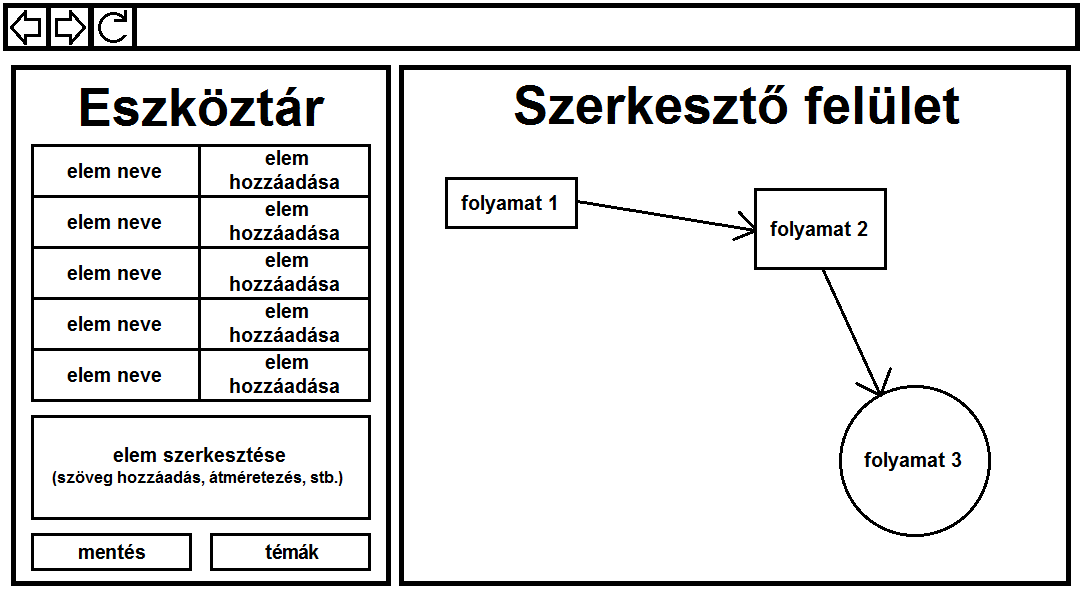
\includegraphics[scale=0.5]{images/sematikus.png}
\caption{A gráfszerkesztő sematikus rajza}
\label{fig:sematikus}
\end{figure}

Az ábra alapján máris van egy elképzelésünk a program szerkezetéről. Nézzük is meg annak konkrét felépítését.

Bal oldalon található az \textbf{eszköztár}, amelynek segítségével különböző funkciók érhetőek el. Innen tudjuk irányítani (létrehozni, szerkeszteni) a gráf felépítéséhez szükséges elemeket. Az eszköztárból az alábbi funkciók érhetőek el:

\begin{enumerate}
\item Az eszköztár nagy részét egy táblázat teszi ki, amely két oszloppal, és a felvihető elemek számával megegyező sorral rendelkezik. A két oszlop a következő jelentéssel bír:

\begin{itemize}
\item Az \textbf{elem neve} rész helyére kerül az adott elem (csomópont) megnevezése. Nevük alapján különböztethetőek meg az egyes elemek. Az elemeket egymás alatt célszerű lehet például használati gyakoriság alapján rendezni (a téglalap, mint tevékenység, az egyik leggyakrabban alkalmazott csomópont típus, ez lehetne legfelül).
\item Az \textbf{elem hozzáadása} felirat helyén az adott elem formája jelenik meg. Ez gyakorlatilag egy gomb, melyre rákattintva hozható létre a mellette feltüntetett nevű elem a szerkesztő felületen egy előre meghatározott helyen. Természetesen ez csak egy alapértelmezett hely, ahol megjelenik kattintás után az adott elem, ezt a későbbiekben lehetőségünk van áthelyezni.
\end{itemize}

\item A táblázat alatt található egy kisebb rész az elemek szerkesztésére. Ez akkor jelenik meg, amikor a szerkesztő felületen rákattintunk egy csomópontra, melyet szerkeszteni szeretnénk. Itt az alábi szerkesztési lehetőségek állnak rendelkezésünkre:

\begin{itemize}
\item \textbf{Szöveget} adhatunk hozzá a kijelölt csomóponthoz. Elegendő csak beírni a felvinni kívánt szöveget, és az azonnal megjelenik az adott csomópont közepén. Ez egységes minden csomópontra (tehát mindegyik típushoz tudunk írni szöveget).
\item \textbf{Átméretezhetjük} a kijelölt elemet. Ez csomópontonként eltérő, hogy milyen paramétereket kíván (például téglalap csomópontnál a szélesség és a hosszúság együttes megadása eredményezi az új méretet, kör alakú csomópont esetében viszont elegendő csak egy paramétert, a sugárt megadni).
\end{itemize}

\item Az eszköztár alatt található egy \textbf{mentés} gomb, melynek segítségével elmenthetjük az elkészített gráfot egy adatbázisba az esetleges későbbi módosítások céljából.

\item Végül a mentés gomb mellett egy \textbf{témák} feliratú gomb helyezkedik el, melyre rákattintva választhatjuk ki az elemek különböző témáját, stílusát. Ez egy apróbb felhasználóbarát élményt nyújt azáltal, hogy különböző színű és alakú formák használatát is lehetővé teszi az alapértelmezetteken kívül. Természetesen ez nem folyásolja be a program használatát, csupán a kinézetét változtatja meg a felhasználó általt kívántra.
\end{enumerate}

A \textbf{szerkesztő felület} (vagy más szóval vászon (\textit{canvas})) a létrehozott elemek megjelenítéséért felelős. Kezdetben üres, egyszínű az egész. Ahogy viszont rákattintunk az eszköztárban egy általunk kiválasztott elemre, úgy az megjelenik rajta, és különböző műveleteket tudunk rajta végezni.

\begin{enumerate}
\item Minden létrehozott csomópont egy egyedi azonosítószámot (\textit{ID}-t) kap. Ez alapján lehet őket megkülönböztetni egymástól.

\begin{itemize}
%\item Az ID-t az adott csomópontra való kattintással lehet lekérni. %5. rész
\item Nem kaphat két különböző csomópont ugyanolyan azonosítószámot, annak egyedinek kell lennie.
\item Ha bármilyen attribútuma módosul egy csomópontnak (pozíciója, színe, rajta lévő szövege, stb.), akkor is az ID-jának állandónak kell lennie.
\end{itemize}

\item A csomópontokat tetszés szerint mozgatni lehet a szerkesztő felület teljes területén.

\item A csomópontok között vonalak húzhatóak az egyik végén egy nyíllal.

\begin{itemize}
\item Csak két, általunk kiválasztott csomópontot lehet összekötni vonallal. Megkülönböztetünk \textit{cél}- és \textit{forrás csomópont}ot. Az összekötő vonal végén a nyíl arra az elemre fog mutatni, amelyet később jelölünk ki (tehát a célcsomópontra).
\item Egy csomóponthoz több vonal is tartozhat, amiből a következő pont is következik:
\item Egy csomópont cél- és forrás csomópontként is funkcionálhat.
\item Tehát gyakorlatilag annyi vonal indulhat ki egy csomópontól / érkezhet be egy csomópontba, amennyit csak szeretne a felhasználó.
\end{itemize}

\item Lehetőség van adott csomópont törlésére.

\begin{itemize}
\item Ha már a továbbiakban nincs szükség egy csomópontra, akkor az letörölhető a szerkesztőfelületről.
\item Ilyenkor ha van a csomóponthoz tartozó vonal, akkor az is törlésre kerül (több vonal esetén az összes).
\item A programnak ügyelnie kell arra, hogy egy csomópont törlése után se legyenek a későbbiekben létrehozott csomópontok ID-jai között azonosak.
\end{itemize}

\end{enumerate}

\Section{Miben különbözik az elkészített program a már használatban lévő gráfszerkesztőktől?}

Korábban említettem, hogy a \textit{Draw.io} alkalmazásnak is vannak hiányosságai annak ellenére, hogy rendkívül sok lehetőséget kínál. Most nézzük néhány példát, amik előfordulhatnak akkor, hogyha a felhasználó nem elég körültekintő egy ilyen vagy ehhez hasonló gráfszerkesztő használata közben, és elkövet olyan hibákat a szerkesztés folyamán, amik miatt nem várt eredmény születhet, illetve hogy ezek a hibák miért jelenthetnek problémát.

\begin{enumerate}
\item Nem pontosan köt össze a vonallal két folyamatot.

\begin{itemize}
\item Mivel a Draw.io a vonalakat is a folyamatokhoz hasonló módon kezeli, ezért azt is a felhasználó tetszés szerinti helyre mozgathatja (tehát nem muszáj összekötnie vele két csomópontot, magában is állhat egy vonal). Ezáltal előfordulhat olyan ábra is, aminél a felhasználó a vonal vége és az összekötendő csomópont között figyelmetlenségből egy kis helyet kihagy, így valójában nem kötött össze két folyamatot, ami össze szeretett volna.
\end{itemize}

\item Ha letöröl egy csomópontot, amely össze van kötve egy másikkal, akkor a hozzá tartozó vonal a "levegőben marad", nem fog két meghatározott csomópontot összekötni, ezáltal az alapvető funkciója válik feleslegessé.

\begin{itemize}
\item Az előző ponthoz hasonló probléma merül fel itt is, tehát a vonal nem két csomópont közötti összeköttetést fog megvalósítani.
\end{itemize}

\item Takarásba kerülhet két vagy több csomópont.

\begin{itemize}
\item Előfordulhat ezáltal, hogy nem olvasható el a csomóponton található szöveg teljes egészében, vagy akár az is, hogy egy nagyobb méretű csomópont teljesen eltakar egy kisebb méretűt, ezáltal megfeledkezünk róla. Ha nincs rá szükség, célszerűbb lenne letörölni, ha pedig van, mert például valamilyen információt tartalmaz a rajta található szöveg, akkor a takarás által elveszettnek hihetjük, így megtörténhet az is, hogy még egyszer létrehozzuk, ami felesleges munkát eredményez.
\end{itemize}

\item Nincs legalább egy kezdő- és legalább egy végállapot.

\begin{itemize}
\item Ahhoz, hogy teljes folyamatábrát modellezzünk, szükséges definiálni egy-egy kezdő- és végállapotot.
\end{itemize}

\end{enumerate}

Ezekkel a fent felsorolt, esetlegesen felmerülő hibákkal szemben nézzük meg azt minden egyes pontnál, hogy az elkészített program hogyan igyekszik azokat kiküszöbölni:

\begin{enumerate}
\item Összekötő vonalat csak adott 2 csomópont között lehetséges húzni.

\begin{itemize}
\item Az összekötést a program úgy oldja meg, hogy a felhasználó jelöli ki azt a két csomópontot, amelyet össze szeretne kötni. Ahogy korábban is említettem lesz egy forrás csomópont és egy célcsomópont, e kettő közt fogja kirajzolni a program a vonalat úgy, hogy a célcsomópont felé mutat a vonal végén lévő nyíl.
\end{itemize}

\item Csomópont törlése esetén a hozzákapcsolt vonal is törlésre kerül.

\begin{itemize}
\item Több nyíl esetén az összes törlődik elkerülve ezáltal a vonalak "levegőben maradását".
\end{itemize}

\item A program jelez, hogyha egymásra kerülnek csomópontok.

\begin{itemize}
\item A felhasználót a canvas más színűre változtatásával figyelmezteti a program amiatt, hogy fedésbe került két csomópont.
\end{itemize}

\item Figyelmeztet az alkalmazás ha hiányzik kezdő- vagy végállapot.

\begin{itemize}
\item Az előző ponthoz hasonlóan itt is arról tájékoztatja a felhasználót a program, hogy nem teljes az általa modellezett folyamatábra.
\end{itemize}

\end{enumerate}

A fent említett utóbbi két példa egészen addig fog hibajelzést generálni a felhasználó számára, amíg meg nem szűnteti azokat.

\Section{Egyszerűbb folyamatábra létrehozása lépésről lépésre}

Nézzük meg, hogy az elkészített alkalmazásban a felhasználó hogyan tud létrehozni egy egyszerűbb folyamatbárát. Fontos, hogy ez az alfejezet csak elméletben írja le, hogy hogyan valósítható meg a folyamatmodellezés a program segítségével. Folyamatábrák konkrét létrehozását, használatát, elmentését az 5. fejezet tárgyalja.

A program, ahogy azt a felépítésénél olvashattuk, egy teljesen üres canvas-szal (vászonnal) fogadja a felhasználót kezdetben. Ez maga a szerkesztő felület, ahol a folyamatmodellezés történik, és itt fogjuk látni az elkészített folyamatábránkat végeredményként. Egy egyszerű folyamatábrát az alábbi lépéseket követve tudunk létrehozni (természetesen ezek a lépések csak iránymutatóak, nem kötött sorrendet határoznak meg):

\begin{enumerate}
\item Első lépésben kiválasztjuk azokat az elemeket az eszköztárból, amelyek a modellezéshez szükségesek. Ha teljes folyamatábrát szeretnénk készíteni, akkor célszerű először a kezdő- és a végállapotokat létrehozni (ezek hiányában figyelmeztet minket a program).
\item Ha már tudjuk, hogy nagyjából hány tevékenységet szeretnénk ábrázolni, akkor annak megfelelő számú csomópontot hozzáadhatunk a vászonhoz.

\begin{itemize}
\item Természetesen a későbbiekben módosíthatóak a csomópontok száma újabbak hozzáadásával vagy meglévők törlésével.
\end{itemize}

\item Miután felvittük ezeket az elemeket, elmozgathatjuk azokat egymástól különálló helyekre azért, hogy lássuk mindegyik csomópontot egyszerre az ábrán, és ezáltal be tudjuk határolni, hogy mekkora helyre lesz szükségünk a végső folyamatábránál.

\begin{itemize}
\item Ha nem mozgatjuk el egymásról a csomópontokat, és takarni fogja legalább kettő egymást, akkor az előző alfejezetben a 4. példaként említett figyelmeztetést fogjuk kapni. Ezt elkerülve célszerű minden létrehozott csomópontot azonnal elmozdítani az alapértelmezett helyéről.
\end{itemize}

\item Ezt követően megírhatjuk az egyes csomópontok szövegeit, hogy azok pontosan milyen tevékenységet jelölnek.

\begin{itemize}
\item Igény szerint a csomópontokat át lehet méretezni, de a csomópont automatikusan elkezd szélesedni mielőtt a beleírt karakterek hossza elérné a csomópont széleit.
\end{itemize}

\item Ha ezzel is megvagyunk, célszerű valamilyen szempont alapján (például időrendi sorrend szerint) egymás után elhelyezni a csomópontokat balról jobbra, illetve fentről lefelé.
\item Ezután összekötjük az általunk összekapcsolni kívánt csomópontokat egymással. Ha teljes folyamatábrát szeretnénk kapni, akkor figyeljünk az alábbi szempontokra:

\begin{itemize}
\item Legyen legalább 1-1 kezdő- és végállapot úgy, hogy a kezdőállapotból csak kifelé, a végállapotba pedig csak befelé vezet legalább egy összekötő vonal.
\item Minden csomópontba el lehessen jutni (tehát a kezdő- és a végállapotokat kivéve mindegyik csomópont legalább két másikkal összeköttetésben legyen úgy, hogy legalább egy bevezető és legalább egy kivezető vonal tartozik hozzá).
\item Ne legyen olyan csomópont, amiből már nem lehet végállapotba jutni a vonalakon keresztül.
\end{itemize}
%Ezekért figyelmeztet a program

\item Végül ha minden simítást elvégeztünk a folyamatábránkon (megfelelő méretűekre változtattuk a csomópontokat, az általunk kívánt helyekre mozgattuk őket, stb.) utolsó lépésként már csak el kell azt mentenünk, és készen is vagyunk.
\end{enumerate}

\Section{UX design szempontok a programnál}

Ezen alfejezet megírásához a(z) \cite{uxblog}. forrás blogbejegyzését használtam alapul. Az itt említett szempontok, meghatározások alapján építettem fel ezt a részt, és azt egészítettem ki a dolgozat programjára jellemző tulajdonságokkal, egyéni gondolatokkal.

\SubSection{Mi az a UX design?}

A \textbf{felhasználói élmény tervezés} (\textit{user experience design}, UX design) egy tervezési folyamat, ami a felhasználói elégedettséget hivatott javítani a felhasználó és a termék között azáltal, hogy növeli a használhatóságot, a hozzáférhetőséget és az élményt. Lényegében azt kell megtervezni, hogy az elkészült alkalmazás vagy termék jó benyomást keltsen a felhasználóban bizonyos szempontokat figyelembe véve. Ez azért fontos, mert ha a felhasználó elégedett a termékkel, akkor azt szívesebben, örömmel használja, és a pozitív visszajelzés több szempontból is hasznos tud lenni. A használó számára is élményt nyújt, és a készítő is elégedett lesz a termékével.

Nélkülözhetetlen egy, a UX-szel kapcsolatos fogalmat is megemlíteni: a \textbf{UI}-t. Ez a \textit{user interface} (magyarul: \textbf{felhasználói felület}) rövidítése, amely a program és a felhasználó közötti kommunikációért felelős. Többféle felhasználói felületek létezik (például szöveges, parancssoros, grafikus). Esetünkben \textit{grafikus felhasználói felület}ről beszélhetünk, hiszen a program grafikus (rajzos, szöveges) elemeket tartalmaz, nem kell parancsokat kiadni bizonyos funkciók elérése érdekében.

\SubSection{UX alapkövetelmények}

Nézzük meg, hogy milyen alapkövetelményei vannak a UX-nek egy adott weboldal szemponjából, illetve hogy ezeket az alapkövetelményeknek mennyire felel meg a szakdolgozat programja.

\begin{enumerate}
\item \textbf{Legyen hasznos:} A célközönségnek kell a legnagyobb fókuszban lennie: jelen esetben ez a felhasználók, akik számára készül a program. Ezáltal úgy kell azt megvalósítani, hogy az érdemleges információt tartalmazzon, felkeltse a felhasználó érdeklődését, és így hasznosnak találja a programot.

\begin{itemize}
\item A program hasznosságát az mutatja, hogy az valós szervezeti folyamatok modellezését segíti elő azáltal, hogy lehetővé teszi a folyamatok ábrázolását. Ennek szükségességéről a 2. fejezetben olvashatunk.
\end{itemize}

\item \textbf{Legyen könnyen használható:} Ne legyen túlzsúfolt az oldal, hanem törekedjen az átláthatóságra. Rajta a navigáció legyen következetes és mindenki számára egyértelmű. Ha az alkalmazás nyújtotta lehetőségeket egyszerűen, könnyedén lehet kezelni, az mindenképp pozitív élményt jelent a felhasználó számára.

\begin{itemize}
\item Az alkalmazás nincs túlbonyolítva, kivitelezése átlátható, használata egyszerű. Ami pedig még inkább megkönnyíti a felhasználó eligazodását, hogy a műveletet végrehajtó gombokra ha ráviszi az egérmutatót, akkor azok egy rövid leírást (\textit{tooltip}et) jelenítenek meg számára, amely a könnyebb használatot segíti elő. Például a \textit{mentés} gombnál leírja, hogy mi fog történni annak megnyomása esetén.
\end{itemize}
%tooltip-et megírni a html-ben (title = "asd")
\item \textbf{Legyen kívánatos:} Fontos szempont a testreszabottság. Elvárás lehet a célközönség részéről a kifogástalan esztétikai élmény. Ezáltal lényeges, hogy minél letisztultabb felületet biztosítson az alkalmazás. Nem mindig a legfelkapottabb a célra legmegfelelőbb, viszont kívánatossá teheti a programot.

\begin{itemize}
\item A program ennél az alapkövetelménynél hiányt szenved, ugyanis nem használja a legmodernebb és legnépszerűbb JavaScript könyvtárakat (sőt, egyáltalán nem használ semmilyen könyvtárat). Ugyanakkor megmutatja, hogy az alap JavaScript, HTML Canvas és némi CSS felhasználásával is elkészíthető egy ilyen alkalmazás.
\end{itemize}

\item \textbf{Legyen könnyen kereshető:} Ez az alapkövetelmény azt írja elő, hogy az adott oldalon / alkalmazásban a keresés hatékony legyen. A felhasználók hamar megtalálják azt, amit keresnek, és hogy egyáltalán az adott oldal rendelkezzen a felhasználó számára a keresett információval.

\begin{itemize}
\item Ezt azért teljesíti könnyen a programunk, mert amint betölt az oldal, mindent a szemünk előtt látunk rajta. Alapvetően nincsenek rejtett dolgok, azonnal elkezdhetjük a folyamatmodellezést, minden egyszerűen a kezünk ügyébe kerül. Egyedül a mentés és a csomópont szerkesztés ami bizonyos funkció végrehajtásakor jelenik meg a felhasználó számára, de ezt az 5. fejezet részletesen tárgyalja majd.
\end{itemize}

\item \textbf{Legyen hozzáférhető:} Vagyis mindenki számára elérhető. A blogbejegyzés különös hangsúlyt fektet a fogyatékkal élőkre, hiszen számukra kellene leginkább biztosítani a könnyű kezelhetőséget és használhatóságot. Ennek ellenére mégsem teljesül sok weboldal esetében ez az alapkövetelmény.

\begin{itemize}
\item Az alkalmazásunk, mint ahogy azt a korábbi pontokban is már olvashattuk, egyszerű használatot és könnyű megértést kínál a felhasználó számára. Ezáltal bárki percek alatt megtanulhatja azt kezelni úgy, hogy képes legyen folyamatábrák készítésére.
\end{itemize}

\item \textbf{Legyen megbízható:} Tehát legyen optimális az oldal azáltal, hogy ne csak szép legyen, hanem gyors is. Ne legyenek rajta felesleges hivatkozások, vagy bármi nem oda illő tartalom, hiszen az összezavarhatja a felhasználót, ami azt eredményezheti, hogy nem fogja többször meglátogatni az oldalt. Ezek elkerülése pozitív benyomást kelthet a felhasználóban, hiszen azt találja az oldalon, amit keresett.

\begin{itemize}
\item Nem tartalmaz a program felesleges mondanivalókat, csupán annyi rajta a tartalom, amennyire szükség van, se több, se kevesebb. A gyorsaságát többek között az adja, hogy nem használ semmilyen külső eszközt (például könyvtárat), illetve nem tartalmaz felesleges nagyméretű objektumokat, amik szintén lassíthatják egyes funkciók elérését.
\end{itemize}

\end{enumerate}